\subsection*{Theoretical Background}\label{sec:TheoBackground}
The following paragraph will provide analytical solutions, assuming there is only one particle with a positive charge ($q > 0$).
\subsubsection*{The Penning Trap}\label{sec:penningtrap}
\begin{figure}[H]
    \centering
    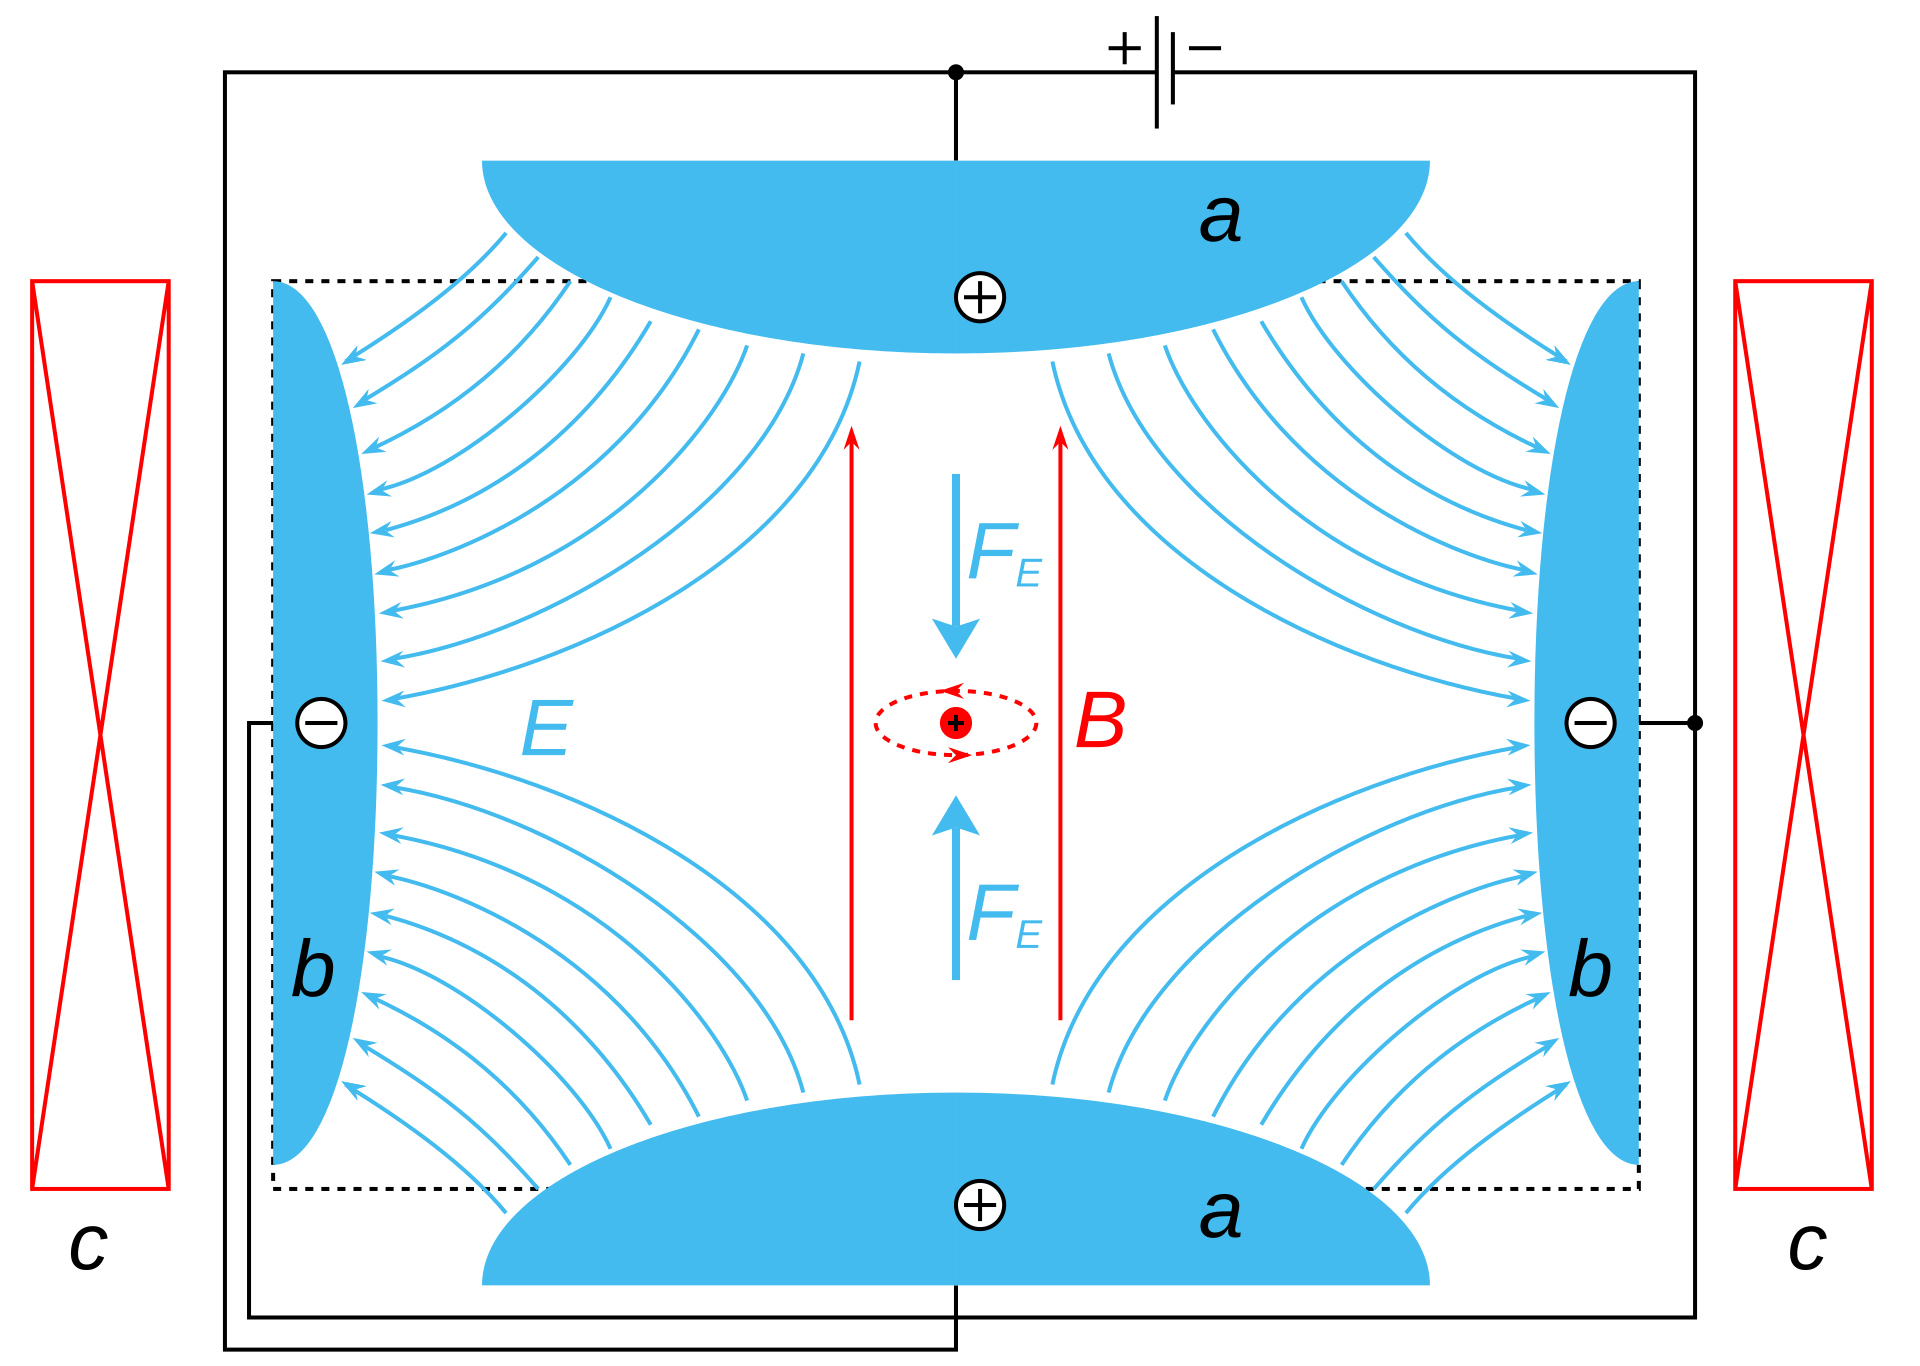
\includegraphics[width = 0.5 \textwidth]{Figures/Penning_Trap.png}
    \caption{Schematic of a Penning trap, further details are provided in \cref{sec:penningtrap}. This illustration is by Arian Kriesch and taken from \url{Wikimedia Commons}}
    \label{fig:penningtrap}
\end{figure}
\Cref{fig:penningtrap} displays a basic schematic for a Penning trap. 
It consists of two positively charged end-cap electrodes (a) and a negatively charged ring electrode (b).
These electrodes generate a static quadrupole electric field (E). The resulting inward electric forces ($F_E$) confine the positively charged particle along the vertical axis. 
Furthermore, external cylindrical magnets (c) produce a strong, uniform magnetic field pointing upwards in the $z$ direction. This field prevents escape by forcing the particle into a continuous orbital trajectory (dashed red path) in the horizontal plane. \cite{PenningTrapbook}\\
The force applied to the particles inside the trap is the Lorentz Force \cite{LectureNotes}:
\begin{align*} \bold{F} = q\bold{E} + q (\bold{v} \times \bold{B}), \end{align*}
In general, the electric field is given as
\begin{align*} \bold{E} = -\nabla(V), \end{align*}
with the potential of the Penning trap \cite{PenningTrapbook}
\begin{align*} V(x,y,z) = \frac{V_0}{2d^2} \cdot (2z^2 -x^2- y^2) \, \text{with} \, d \, = \, \sqrt{z_0^2 + \frac{r_0^2}{2}}, \end{align*}
where $z_0$ is the distance from the centre to the end caps and $r_0$ is the distance from the centre to the ring.)
The electric field is therefore given by:
\begin{align*}
    E_x &= -\frac{\partial}{\partial x}(\frac{V_0}{2d^2} (2z^2 -x^2-y^2) = \frac{V_0}{d^2} \cdot x, \\
    E_y &= -\frac{\partial}{\partial y}(\frac{V_0}{2d^2} (2z^2 -x^2-y^2) = \frac{V_0}{d^2} \cdot y, \\
    E_z &= -\frac{\partial}{\partial z}(\frac{V_0}{2d^2} (2z^2 -x^2-y^2) = \frac{-2V_0}{d^2} \cdot z.
\end{align*}
As the Lorentz Force is the only force acting upon the particle, Newton's second law for one particle with charge $q$ can be written as:
\begin{itemize}
    \item $\mathbf{x-direction}$:
    \begin{align}\label{eq:xdirect}
        m\ddot{x} &= qE_x + q(\mathbf{v} \times \mathbf{B})_x \notag \\
        m\ddot{x} &= qE_x + q\dot{y}B_0 \notag \\
        m\ddot{x} &= q\frac{V_0}{d^2}x + q\dot{y}B_0 \notag \\
        \Leftrightarrow 0 &= \ddot{x} - \frac{qV_0}{md^2}x - \frac{qB_0}{m}\dot{y} = \ddot{x} - \frac{1}{2}\omega_z^2 x - \omega_0 \dot{y}.
    \end{align}

    \item $\mathbf{y-direction}$:
    \begin{align}\label{eq:ydirect}
        m\ddot{y} &= qE_y - q\dot{x}B_0 \notag \\
        m\ddot{y} &= q\frac{V_0}{d^2}y - q\dot{x}B_0 \notag \\
        \Leftrightarrow 0 &= \ddot{y} - \frac{qV_0}{md^2}y + \frac{qB_0}{m}\dot{x} = \ddot{y} - \frac{1}{2}\omega_z^2 y + \omega_0 \dot{x}.
    \end{align}

    \item $\mathbf{z-direction}$:
    \begin{align}\label{eq:zdirect}
        m\ddot{z} &= qE_z + 0 \notag \\
        \Leftrightarrow 0 &= \ddot{z} + \frac{2qV_0}{md^2}z \notag \\
        0 &= \ddot{z} + \omega_z^2 z.
    \end{align}
\end{itemize}
For simplicity, we define $\omega_z^2 = \frac{2qV_0}{md^2}$ and $\omega_0 = \frac{qB_0}{m}$.
The solution for the z-direction is well-known as it is a harmonic oscillator with the general solution:
\begin{align} \label{eq: zana} z = A \cdot \cos{\omega_z t} + B \cdot \sin{\omega_z t}. \end{align}
Here, the constants $A$ and $B$ have to be calculated from the given initial conditions for the respective particle.
Our simulations will include both the starting position $\bold{r}$ and the starting velocity $\bold{v}$ as initial conditions.
From these, we can calculate the two constants using the z-components of the respective vectors by substituting $t=0$ into \cref{eq: zana}.
\begin{equation*}
    z(t=0) = A,
\end{equation*}
\begin{equation*}
    \frac{dz(t=0)}{dt} = B \omega_z.
\end{equation*}
To solve the DEs for the other directions we introduce a new complex-valued function $f(t) = x(t) + iy(t)$, with the first and second derivative $\dot{f(t)} = \dot{x(t)} + i\dot{y(t)}$ and $\ddot{f(t)} = \ddot{x(t)} + i\ddot{y(t)}$.
Adding \cref{eq:xdirect} and $i$ times \cref{eq:ydirect}, we find the following form:
\begin{align*} \ddot{x} + i\ddot{y} + \omega_0(i\dot{x} - \dot{y}) -\frac{1}{2}\omega_z^2 (x + iy) = 0. \end{align*}
This can be associated with the introduced function $f(t)$, the final form is then:
\begin{align}\label{eq:finalform} \ddot{f{t}} + i\omega_0 \dot{f(t)} - \frac{1}{2} \omega_z^2 f(t) = 0. \end{align}
To solve \cref{eq:finalform}, we choose a complex ansatz of the form
\begin{equation} \label{eq:Analyticalxy}
    f(t) = A_+ e^{-i(\omega_+ t + \phi_+)} + A_- e^{-i(\omega_- t + \phi_-)},  
\end{equation}
where $\phi_+$ and $\phi_-$ are constant phases, the amplitudes $A_+$ and $A_-$ are positive, and
\begin{align}\label{eq:omegapm}\omega_\pm = \frac{\omega_0 \pm \sqrt{\omega_0^2 - 2\omega_z^2}}{2}.\end{align}
The two rotary motions, whose superposition make up this analytical solution in the x and y coordinates, are usually called the magnetron drift ($\omega_-$ rotation) and the cyclotron motion ($\omega_+$ rotation)\cite{PenningTrapbook}.
The physical coordinates are found as $x(t) = \text{Re} (f(t))$ and $y(t) = \text{Im} (f(t))$.
To find a realistic solution, we have to pay attention to the following restriction: 
The solution of $f(t)$ should remain bounded even for high values for $t$ ($|f(t)| < \infty \text{ for } t \rightarrow \infty$).
The constraint on $\omega_{\pm}$ for containment is that it has to be a real number. Elsewhere, the exponent will not be complex anymore for one summand (because we could write then $\omega_{\pm}$ as a complex number of the form $a+ib$ and as $i \cdot i$ is real one exponent looks like $e^{bt}$). To avoid this, the square root in \cref{eq:omegapm} has to be positive. Thus, $$\omega_0^2 > 2\omega_z^2$$ has to hold \cite{PenningTrapbook}. Written in terms of the constants given by the Penning trap configuration, this leads to \cref{eq:stability}.
\begin{equation} \label{eq:stability}
    \frac{q}{m} > \frac{4V_0}{d^2B_0^2}.
\end{equation}
To calculate the distance from the particle to the origin inside the x-y plane, we will use the triangle inequality to approximate the maximum as well as the minimum value. For every time, we know:
$$R(t) = |f(t)| = |A_+ e^{-i(\omega_+ t + \phi_+)} + A_- e^{-i(\omega_- t + \phi_-)}|.$$
For the upper bound, we use the triangle inequality:
\begin{align*}
R(t) &\le |A_+ e^{-i(\omega_+ t + \phi_+)}| + |A_- e^{-i(\omega_- t + \phi_-)}| \\
&= |A_+| + |A_-| = A_+ + A_- = R_+.
\end{align*}
For the lower bound, we use the reverse triangle inequality:
\begin{align*} 
R(t) &\ge ||A_+ e^{-i(\omega_+ t + \phi_+)}| - |A_- e^{-i(\omega_- t + \phi_-)}|| \\
&= ||A_+| - |A_-|| = |A_+ - A_-| = R_-. \end{align*}
For further tests in \cref{sec:results_and_discussion}, we need to introduce initial conditions in order to find a specific analytic solution. In our first investigation, using only a single particle, these are given by:
\begin{align}
    \centering
    x(0) &= x_0 > 0 &\text{ and } \dot{x}(0) &= 0, \\
    y(0) &= 0 &\text{ and } \dot{y}(0) &= v_0 > 0, \\
    z(0) &= z_0 &\text{ and } \dot{z}(0) &= 0.
\end{align}
Thus (see \cref{eq:zdirect}):
\begin{align*}
    z(t) = z_0 \cos{\omega_zt}.
\end{align*}
Considering a movement in the $xy$-plane, a specific solution is given by \cref{eq:finalform} with:
\begin{align*}
    A_+ &= \frac{v_0 + \omega_- x_0}{\omega_+ - \omega_-}\footnotemark, & A_- &= \frac{v_0 + \omega_+ x_0}{\omega_+ - \omega_-}, \\[10pt]
    \phi_+ &= \pi, & \phi_- &= 0.
\end{align*}
\footnotetext{For general initial conditions, the amplitudes and the phases are moduli and negative arguments of complex numbers.}
For $n$ particles with charges $\{q_1, ... , q_n\}$ and masses $\{m_1, ... , m_n\}$ the differential equations have the following form:
\begin{align*}
    \ddot{x}_i - \omega_{0,i} \dot{y}_i - \frac{1}{2} \omega_{z,i}^2 x_i - k_e \frac{q_i}{m_i} \sum_{j \neq i} q_j \frac{x_i - x_j}{|\mathbf{r}_i - \mathbf{r}_j|^3} &= 0, \\[10pt]
    \ddot{y}_i + \omega_{0,i} \dot{x}_i - \frac{1}{2} \omega_{z,i}^2 y_i - k_e \frac{q_i}{m_i} \sum_{j \neq i} q_j \frac{y_i - y_j}{|\mathbf{r}_i - \mathbf{r}_j|^3} &= 0, \\[10pt]
    \ddot{z}_i + \omega_{z,i}^2 z_i - k_e \frac{q_i}{m_i} \sum_{j \neq i} q_j \frac{z_i - z_j}{|\mathbf{r}_i - \mathbf{r}_j|^3} &= 0.
\end{align*}
The Coulomb force couples the equations for two or more particles, leading to non-linear dynamics, which are generally difficult to solve analytically. 
Instead, researchers have relied on numerical methods to study this system, as was done in e.g. \cite{NumericalPenning1}.
Here, we introduce numerical approaches such as RK4 and FE to treat this coupled system of equations. 
However, both of them are expecting a first-order DE. The associated first-order DEs are:
\begin{align} \label{eq: coupledstart}
    \centering
    \dot{x}_i &= v_{x,i}, \\
    \dot{y}_i &= v_{y,i}, \\
    \dot{z}_i &= v_{z,i}, \\
    \dot{v}_{x,i} &= \omega_{0,i} v_{y,i} + \frac{1}{2} \omega_{z,i}^2 x_i + k_e \frac{q_i}{m_i} \sum_{j \neq i} q_j \frac{x_i - x_j}{|\mathbf{r}_i - \mathbf{r}_j|^3}, \label{eq:vstart} \\[8pt] 
    \dot{v}_{y,i} &= -\omega_{0,i} v_{x,i} + \frac{1}{2} \omega_{z,i}^2 y_i + k_e \frac{q_i}{m_i} \sum_{j \neq i} q_j \frac{y_i - y_j}{|\mathbf{r}_i - \mathbf{r}_j|^3}, \\[8pt]
    \dot{v}_{z,i} &= -\omega_{z,i}^2 z_i + k_e \frac{q_i}{m_i} \sum_{j \neq i} q_j \frac{z_i - z_j}{|\mathbf{r}_i - \mathbf{r}_j|^3}. \label{eq: coupledend}
\end{align}
Unless indicated otherwise, our simulation results and the associated code use the following configurations:
\begin{equation*}
    B_0 = 1.00\,\mathrm{T} \simeq 9.65 \times 10^1 \, \frac{\mathrm{u}}{(\mathrm{\mu s}) \, \mathrm{e}},
\end{equation*}
\begin{equation*}
    V_0 = 25.0\,\mathrm{mV} \simeq 2.41 \times 10^6 \, \frac{\mathrm{u} \, (\mathrm{\mu m})^2}{(\mathrm{\mu s})^2 \, \mathrm{e}},
\end{equation*}
\begin{equation*}
    d = 500\,\mathrm{\mu m}.
\end{equation*}
The particles we simulate are singly-charged \(\ce{^{40}Ca}\) ions. We chose to use this particular isotope, as it is the most abundant naturally occurring \(\ce{Ca}\) isotope. \cite{CAWeight} Therefore the weight of the particles will be: $m = 39.962 590 863 u$.
Given these constants, we can predict if the constructed Penning trap can contain a single \(\ce{^{40}Ca}\) ion stably by using \cref{eq:stability}.
\begin{equation*}
    \frac{1 e}{39.962 590 863 u} > \frac{4 \cdot 2.41 \cdot 10^6 \, \frac{\mathrm{u} \, (\mathrm{\mu m})^2}{(\mathrm{\mu s})^2 \, \mathrm{e}}}{\left (500 \mu m \cdot 9.65 \times 10^1 \, \frac{\mathrm{u}}{(\mathrm{\mu s}) \, \mathrm{e}} \right)^2}
\end{equation*}
\begin{equation*}
    0.0250234026 > 4.140782303 \cdot 10^{-3}
\end{equation*}
Therefore, we expect our simulation to show that a single particle stays contained inside the trap.
